% ------------------------------------------------------------
% LaTeX Template für die DHBW zum Schnellstart!
% Original: https://github.wdf.sap.corp/vtgermany/LaTeX-Template-DHBW
% ------------------------------------------------------------
% ---- Präambel mit Angaben zum Dokument
\documentclass[
	fontsize=12pt,           % Leitlinien sprechen von Schriftgröße 12.
	paper=A4,
	twoside=false,
	listof=totoc,            % Tabellen- und Abbildungsverzeichnis ins Inhaltsverzeichnis
	bibliography=totoc,      % Literaturverzeichnis ins Inhaltsverzeichnis aufnehmen
	titlepage,               % Titlepage-Umgebung anstatt \maketitle
	headsepline,             % horizontale Linie unter Kolumnentitel
	abstract,              % Überschrift einschalten, Abstract muss in {abstract}-Umgebung stehen
]{scrreprt}                  % Verwendung von KOMA-Report
\usepackage[utf8]{inputenc}  % UTF8 Encoding einschalten
\usepackage[ngerman]{babel}  % Neue deutsche Rechtschreibung
\usepackage[T1]{fontenc}     % Ausgabe von westeuropäischen Zeichen (auch Umlaute)
\usepackage{microtype}       % Trennung von Wörtern wird besser umgesetzt
\usepackage{lmodern}         % Nicht-gerasterte Schriftarten (bei MikTeX erforderlich)
\usepackage{graphicx}        % Einbinden von Grafiken erlauben
\usepackage{wrapfig}         % Grafiken fließend im Text
\usepackage{setspace}        % Zeilenabstand \singlespacing, \onehalfspaceing, \doublespacing
\usepackage[
	%showframe,                % Ränder anzeigen lassen
	left=2.7cm, right=2.5cm,
	top=2.5cm,  bottom=2.5cm,
	includeheadfoot
]{geometry}                      % Seitenlayout einstellen
\usepackage{scrlayer-scrpage}    % Gestaltung von Fuß- und Kopfzeilen
\usepackage{acronym}             % Abkürzungen, Abkürzungsverzeichnis
\usepackage{titletoc}            % Anpassungen am Inhaltsverzeichnis
\contentsmargin{0.75cm}          % Abstand im Inhaltsverzeichnis zw. Punkt und Seitenzahl
\usepackage[                     % Klickbare Links (enth. auch "nameref", "url" Package)
  hidelinks,                     % Blende die "URL Boxen" aus.
  breaklinks=true                % Breche zu lange URLs am Zeilenende um
]{hyperref}
\usepackage[hypcap=true]{caption}% Anker Anpassung für Referenzen
\urlstyle{same}                  % Aktuelle Schrift auch für URLs
% Anpassung von autoref für Gleichungen (ergänzt runde Klammern) und Algorithm.
% Anstatt "Listing" kann auch z.B. "Code-Ausschnitt" verwendet werden. Dies sollte
% jedoch synchron gehalten werden mit \lstlistingname (siehe weiter unten).
\addto\extrasngerman{%
	\def\equationautorefname~#1\null{Gleichung~(#1)\null}
	\def\lstnumberautorefname{Zeile}
	\def\lstlistingautorefname{Listing}
	\def\algorithmautorefname{Algorithmus}
	% Damit einheitlich "Abschnitt 1.2[.3]" verwendet wird und nicht "Unterabschnitt 1.2.3"
	% \def\subsectionautorefname{Abschnitt}
}

% ---- Abstand verkleinern von der Überschrift 
\renewcommand*{\chapterheadstartvskip}{\vspace*{.5\baselineskip}}

% Hierdurch werden Schusterjungen und Hurenkinder vermieden, d.h. einzelne Wörter
% auf der nächsten Seite oder in einer einzigen Zeile.
% LaTeX kann diese dennoch erzeugen, falls das Layout ansonsten nicht umsetzbar ist.
% Diese Werte sind aber gute Startwerte.
\widowpenalty10000
\clubpenalty10000

% ---- Für das Quellenverzeichnis
\usepackage[
	backend = biber,                % Verweis auf biber
	language = auto,
	style = alphabetic,                % Nummerierung der Quellen mit Zahlen
	sorting = anyt,                 % none = Sortierung nach der Erscheinung im Dokument
	sortcites = true,               % Sortiert die Quellen innerhalb eines cite-Befehls
	block = space,                  % Extra Leerzeichen zwischen Blocks
	hyperref = true,                % Links sind klickbar auch in der Quelle
	%backref = true,                % Referenz, auf den Text an die zitierte Stelle
	bibencoding = auto,
	giveninits = true,              % Vornamen werden abgekürzt
	doi=false,                      % DOI nicht anzeigen
	isbn=false,                     % ISBN nicht anzeigen
    alldates=short                  % Datum immer als DD.MM.YYYY anzeigen
]{biblatex}
\addbibresource{Inhalt/literatur.bib}
\setcounter{biburlnumpenalty}{3000}     % Umbruchgrenze für Zahlen
\setcounter{biburlucpenalty}{6000}      % Umbruchgrenze für Großbuchstaben
\setcounter{biburllcpenalty}{9000}      % Umbruchgrenze für Kleinbuchstaben
\DeclareNameAlias{default}{family-given}  % Nachname vor dem Vornamen
\AtBeginBibliography{\renewcommand{\multinamedelim}{\addslash\space
}\renewcommand{\finalnamedelim}{\multinamedelim}}  % Schrägstrich zwischen den Autorennamen
\DefineBibliographyStrings{german}{
  urlseen = {Einsichtnahme:},                      % Ändern des Titels von "besucht am"
}
\usepackage[babel,german=quotes]{csquotes}         % Deutsche Anführungszeichen + Zitate


% ---- Für Mathevorlage
\usepackage{amsmath}    % Erweiterung vom Mathe-Satz
\usepackage{amssymb}    % Lädt amsfonts und weitere Symbole
\usepackage{MnSymbol}   % Für Symbole, die in amssymb nicht enthalten sind.


% ---- Für Quellcodevorlage
\usepackage{scrhack}                    % Hack zur Verw. von listings in KOMA-Script
\usepackage{listings}                   % Darstellung von Quellcode
\usepackage{xcolor}                     % Einfache Verwendung von Farben
% -- Eigene Farben für den Quellcode
\definecolor{JavaLila}{rgb}{0.4,0.1,0.4}
\definecolor{JavaGruen}{rgb}{0.3,0.5,0.4}
\definecolor{JavaBlau}{rgb}{0.0,0.0,1.0}
\definecolor{ABAPKeywordsBlue}{HTML}{6000ff}
\definecolor{ABAPCommentGrey}{HTML}{808080}
\definecolor{ABAPStringGreen}{HTML}{4da619}
\definecolor{PyKeywordsBlue}{HTML}{0000AC}
\definecolor{PyCommentGrey}{HTML}{808080}
\definecolor{PyStringGreen}{HTML}{008080}
% -- Farben für ABAP CDS
\definecolor{CDSString}{HTML}{FF8C00}
\definecolor{CDSKeywords}{HTML}{6000ff}
\definecolor{CDSAnnotation}{HTML}{00BFFF}
\definecolor{CDSComment}{HTML}{808080}
\definecolor{CDSFunc}{HTML}{FF0000}
% -- Farben für SQL
\definecolor{SQLString}{HTML}{15ABF6}
\definecolor{SQLKeywords}{HTML}{7B30FF}
\definecolor{SQLVariables}{HTML}{000000}

% -- Default Listing-Styles

\lstset{
	% Das Paket "listings" kann kein UTF-8. Deswegen werden hier 
	% die häufigsten Zeichen definiert (ä,ö,ü,...)
	literate=%
		{á}{{\'a}}1 {é}{{\'e}}1 {í}{{\'i}}1 {ó}{{\'o}}1 {ú}{{\'u}}1
		{Á}{{\'A}}1 {É}{{\'E}}1 {Í}{{\'I}}1 {Ó}{{\'O}}1 {Ú}{{\'U}}1
		{à}{{\`a}}1 {è}{{\`e}}1 {ì}{{\`i}}1 {ò}{{\`o}}1 {ù}{{\`u}}1
		{À}{{\`A}}1 {È}{{\'E}}1 {Ì}{{\`I}}1 {Ò}{{\`O}}1 {Ù}{{\`U}}1
		{ä}{{\"a}}1 {ë}{{\"e}}1 {ï}{{\"i}}1 {ö}{{\"o}}1 {ü}{{\"u}}1
		{Ä}{{\"A}}1 {Ë}{{\"E}}1 {Ï}{{\"I}}1 {Ö}{{\"O}}1 {Ü}{{\"U}}1
		{â}{{\^a}}1 {ê}{{\^e}}1 {î}{{\^i}}1 {ô}{{\^o}}1 {û}{{\^u}}1
		{Â}{{\^A}}1 {Ê}{{\^E}}1 {Î}{{\^I}}1 {Ô}{{\^O}}1 {Û}{{\^U}}1
		{œ}{{\oe}}1 {Œ}{{\OE}}1 {æ}{{\ae}}1 {Æ}{{\AE}}1 {ß}{{\ss}}1
		{ű}{{\H{u}}}1 {Ű}{{\H{U}}}1 {ő}{{\H{o}}}1 {Ő}{{\H{O}}}1
		{ç}{{\c c}}1 {Ç}{{\c C}}1 {ø}{{\o}}1 {å}{{\r a}}1 {Å}{{\r A}}1
		{€}{{\euro}}1 {£}{{\pounds}}1 {«}{{\guillemotleft}}1
		{»}{{\guillemotright}}1 {ñ}{{\~n}}1 {Ñ}{{\~N}}1 {¿}{{?`}}1,
	breaklines=true,        % Breche lange Zeilen um 
	breakatwhitespace=true, % Wenn möglich, bei Leerzeichen umbrechen
	% Symbol für Zeilenumbruch einfügen
	prebreak=\raisebox{0ex}[0ex][0ex]{\ensuremath{\rhookswarrow}},
	postbreak=\raisebox{0ex}[0ex][0ex]{\ensuremath{\rcurvearrowse\space}},
	tabsize=4,                                 % Setze die Breite eines Tabs
	basicstyle=\ttfamily\small,                % Grundsätzlicher Schriftstyle
	columns=fixed,                             % Besseres Schriftbild
	numbers=left,                              % Nummerierung der Zeilen
	%frame=single,                             % Umrandung des Codes
	showstringspaces=false,                    % Keine Leerzeichen hervorheben
	keywordstyle=\color{blue},
	ndkeywordstyle=\bfseries\color{darkgray},
	identifierstyle=\color{black},
	commentstyle=\itshape\color{JavaGruen},   % Kommentare in eigener Farbe
	stringstyle=\color{JavaBlau},             % Strings in eigener Farbe,
	captionpos=b,                             % Bild*unter*schrift
	xleftmargin=5.0ex
}

% ---- Eigener JAVA-Style für den Quellcode
\renewcommand{\ttdefault}{pcr}               % Schriftart, welche auch fett beinhaltet
\lstdefinestyle{EigenerJavaStyle}{
	language=Java,                             % Syntax Highlighting für Java
	%frame=single,                             % Umrandung des Codes
	keywordstyle=\bfseries\color{JavaLila},    % Keywords in eigener Farbe und fett
	commentstyle=\itshape\color{JavaGruen},    % Kommentare in eigener Farbe und italic
	stringstyle=\color{JavaBlau}               % Strings in eigener Farbe
}

% ---- Eigener ABAP-Style für den Quellcode
\renewcommand{\ttdefault}{pcr}
\lstdefinestyle{EigenerABAPStyle}{
	language=[R/3 6.10]ABAP,
	morestring=[b]\|,                          % Für Pipe-Strings
	morestring=[b]\`,                          % für Backtick-Strings
	keywordstyle=\bfseries\color{ABAPKeywordsBlue},
	commentstyle=\itshape\color{ABAPCommentGrey},
	stringstyle=\color{ABAPStringGreen},
	tabsize=2,
	morekeywords={
		types,
		@data,
		as,
		lower,
		start,
		selection,
		order,
		by,
		inner,
		join,
		key,
		end,
		cast
	}
}

% ---- Eigener SQL-Style für den Quellcode
\renewcommand{\ttdefault}{pcr}
\lstdefinestyle{EigenerSQLStyle}{
	language=SQL,
	keywordstyle=\bfseries\color{SQLKeywords},
	commentstyle=\itshape\color{ABAPCommentGrey},
	stringstyle=\color{SQLString},
	morekeywords={
		SELECT,
		INSERT,
		CREATE,
		UPDATE,
		MOVE,
		AS,
		ON,
		COUNT,
		MAX,
		MIN,
		DELETE,
		GRANT,
		PERMISSIONS,
		ALL,
		REVOKE,
		INNER JOIN,
		RIGHT JOIN,
		LEFT JOIN,
		FULL JOIN,
		FULL OUTER JOIN,
		CROSS JOIN,
		IS,
		NULL,
		DISTINCT,
		JOIN
	}
}

% ---- Eigener Python-Style für den Quellcode
\renewcommand{\ttdefault}{pcr}
\lstdefinestyle{EigenerPythonStyle}{
	language=Python,
	columns=flexible,
	keywordstyle=\bfseries\color{PyKeywordsBlue},
	commentstyle=\itshape\color{PyCommentGrey},
	stringstyle=\color{PyStringGreen}
}

%----- ABAP-CDS-View language
\lstdefinelanguage{ABAPCDS}{
	sensitive=false,
	%Keywords
	morekeywords={define,
		view,
		as,
		select,
		from,
		inner,
		join,
		on,
		key,
		case,
		when,
		then,
		else,
		end,
		true,
		false,
		cast,
		where,
		and,
		distinct,
		group,
		by,
		having,
		min,
		sum,
		max,
		count,
		avg
	},
	%Methoden
	morekeywords=[2]{
		div,
		currency\_conversion,
		dats\_days\_between,
		concat\_with\_space,
		dats\_add_days,
		dats\_is\_valid,
		dats\_add\_months,
		unit\_conversion,
		division,
		mod,
		abs,
		floor,
		ceil,
		round,
		concat,
		replace,
		substring,
		left,
		right,
		length
	},
	morecomment=[s][\color{CDSAnnotation}]{@}{:},
	morecomment=[l][\itshape\color{CDSComment}]{//},
	morecomment=[s][\itshape\color{CDSComment}]{/*}{*/},
	morestring=[b][\color{CDSString}]',
	keywordstyle=\bfseries\color{CDSKeywords},
	keywordstyle=[2]\color{CDSFunc}
}

  % Weitere Details sind ausgelagert

\usepackage{algorithm}                  % Für Algorithmen-Umgebung (ähnlich wie lstlistings Umgebung)
\usepackage{algpseudocode}              % Für Pseudocode. Füge "[noend]" hinzu, wenn du kein "endif",
                                        % etc. haben willst.

\makeatletter                           % Sorgt dafür, dass man @ in Namen verwenden kann.
                                        % Ansonsten gibt es in der nächsten Zeile einen Compilefehler.
\renewcommand{\ALG@name}{Algorithmus}   % Umbenennen von "Algorithm" im Header der Listings.
\makeatother                            % Zeichen wieder zurücksetzen
\renewcommand{\lstlistingname}{Code} % Erlaubt das Umbenennen von "Listing" in anderen Titel.

% ---- Tabellen
\usepackage{booktabs}  % Für schönere Tabellen. Enthält neue Befehle wie \midrule
\usepackage{multirow}  % Mehrzeilige Tabellen
\usepackage{siunitx}   % Für SI Einheiten und das Ausrichten Nachkommastellen
\sisetup{locale=DE, range-phrase={~bis~}, output-decimal-marker={,}} % Damit ein Komma und kein Punkt verwendet wird.
\usepackage{xfrac} % Für siunitx Option "fraction-function=\sfrac"

% ---- Für Definitionsboxen in der Einleitung
\usepackage{amsthm}                     % Liefert die Grundlagen für Theoreme
\usepackage[framemethod=tikz]{mdframed} % Boxen für die Umrandung
% ---- Definition für Highlight Boxen

% ---- Grundsätzliche Definition zum Style
\newtheoremstyle{defi}
  {\topsep}         % Abstand oben
  {\topsep}         % Abstand unten
  {\normalfont}     % Schrift des Bodys
  {0pt}             % Einschub der ersten Zeile
  {\bfseries}       % Darstellung von der Schrift in der Überschrift
  {:}               % Trennzeichen zwischen Überschrift und Body
  {.5em}            % Abstand nach dem Trennzeichen zum Body Text
  {\thmname{#3}}    % Name in eckigen Klammern
\theoremstyle{defi}

% ------ Definition zum Strich vor eines Texts
\newmdtheoremenv[
  hidealllines = true,       % Rahmen komplett ausblenden
  leftline = true,           % Linie links einschalten
  innertopmargin = 0pt,      % Abstand oben
  innerbottommargin = 4pt,   % Abstand unten
  innerrightmargin = 0pt,    % Abstand rechts
  linewidth = 3pt,           % Linienbreite
  linecolor = gray!40,       % Linienfarbe
]{defStrich}{Definition}     % Name der des formats "defStrich"

% ------ Definition zum Eck-Kasten um einen Text
\newmdtheoremenv[
  hidealllines = true,
  innertopmargin = 6pt,
  linecolor = gray!40,
  singleextra={              % Eck-Markierungen für die Definition
    \draw[line width=3pt,gray!50,line cap=rect] (O|-P) -- +(1cm,0pt);
    \draw[line width=3pt,gray!50,line cap=rect] (O|-P) -- +(0pt,-1cm);
    \draw[line width=3pt,gray!50,line cap=rect] (O-|P) -- +(-1cm,0pt);
    \draw[line width=3pt,gray!50,line cap=rect] (O-|P) -- +(0pt,1cm);
  }
]{defEckKasten}{Definition}  % Name der des formats "defEckKasten"  % Weitere Details sind ausgelagert

% ---- Für Todo Notes
\usepackage{todonotes}
\setlength {\marginparwidth }{2cm}      % Abstand für Todo Notizen

\usepackage{pdfpages}
\usepackage{jslistings}

% ---- Elektronische Version oder Gedruckte Version?
% ---- Unterschied: Die elektronische Version enthält keinen Platzhalter für die Unterschrift
\usepackage{ifthen}
\newboolean{e-Abgabe}
\setboolean{e-Abgabe}{true}    % false=gedruckte Fassung

% ---- Persönlichen Daten:
\newcommand{\titel}{Integrationsseminar}
\newcommand{\titelheader}{Integrationsseminar}
\newcommand{\arbeit}{Assignment}
\newcommand{\studiengang}{Wirtschaftsinformatik: Software Engineering}
\newcommand{\studienjahr}{2022}
\newcommand{\autor}{Mathis Neunzig}
\newcommand{\autorReverse}{Neunzig, Mathis}
\newcommand{\verfassungsort}{Walldorf}
\newcommand{\matrikelnr}{2240587}
\newcommand{\kurs}{WI 2020 MA SE B}
\newcommand{\bearbeitungsmonat}{Juni 2023}
\newcommand{\abgabe}{15. Juni 2023}
\newcommand{\bearbeitungszeitraum}{07.06.23 - 15.06.23}
\newcommand{\dozent}{Alexander Lütke}
\newcommand{\firmaName}{SAP SE}
\newcommand{\firmaStrasse}{Dietmar-Hopp-Allee 16}
\newcommand{\firmaPlz}{69190 Walldorf, Deutschland}
\newcommand{\betreuerFirma}{Joscha-Philipp Bohn}
\newcommand{\betreuerDhbw}{Prof. Dr. Thomas Holey}

% ---- Adressen:
\newcommand{\sapdeName}{SAP Deutschland SE und Co. KG}
\newcommand{\sapdeStrasse}{Hasso-Plattner-Ring 7}
\newcommand{\sapdePLZ}{69190 Walldorf, Deutschland}
\newcommand{\aribaName}{Ariba Inc. (SAP Ariba)}
\newcommand{\aribaStrasse}{3420 Hillview Ave}
\newcommand{\aribaPLZ}{CA 94304 Palo Alto, USA}
\newcommand{\concurName}{Concur Technologies Inc., Concur Holdings (Netherlands) B.V. (SAP Concur)}
\newcommand{\concurStrasse}{601 108th Ave NE}
\newcommand{\concurPLZ}{WA 98004 Bellevue, USA}
\newcommand{\fgName}{SAP America Inc., SAP Fieldglass, SAP SuccessFactors}
\newcommand{\fgStrasse}{3999 West Chester Pike}
\newcommand{\fgPLZ}{PA 19073 Newtown Square, USA}
\newcommand{\hybrisName}{hybris AG (SAP Hybris)}
\newcommand{\hybrisStrasse}{Birkenstrasse 49}
\newcommand{\hybrisPLZ}{6343 Rotkreuz, Schweiz}
\newcommand{\gName}{Gartner Inc.}
\newcommand{\gStrasse}{56 Top Gallant Road}
\newcommand{\gPLZ}{Stamford, CT 06902 USA}

% ---- Metainformation für das PDF Dokument
\hypersetup{
	pdftitle    = {\titel},
	pdfsubject  = {\arbeit},
	pdfauthor   = {\autor},
	%pdfkeywords = {Keywords angeben},
	pdfcreator  = {LaTeX},
	%pdfproducer = {in der Regel pdfTeX}
}

% ---- Definition der Kopf- und Fußzeilen
\clearpairofpagestyles                          % Löschen von LaTeX Standard
\automark[section]{chapter}                     % Füllen von section und chapter
\renewcommand*{\chaptermarkformat}{}            % Entfernt die Kapitelnummer
\renewcommand*{\sectionmarkformat}{}            % Entfernt die Sectionnummer
% Angaben [für "plain"]{für "scrheadings"}
\ihead[]{\titelheader}                          % Kopfzeile links
\chead[]{}                                      % Kopfzeile mitte
\ohead[]{\rightmark}                            % Kopfzeile rechts
\ifoot[]{}                                      % Fußzeile links
\cfoot*{\sffamily\pagemark}                     % Fußzeile mitte
\ofoot[]{}                                      % Fußzeile rechts
\KOMAoptions{
   headsepline = 0.2pt,                         % Liniendicke Kopfzeile
   footsepline = false                          % Liniendicke Fußzeile
}


% ---- Hilfreiches
\newcommand{\zB}{z.\,B. }   % "z.B." mit kleinem Leeraum dazwischen (ohne wäre nicht korrekt)
\newcommand{\dash}{d.\,h. }

\newcommand{\code}[1]{\texttt{#1}} % Ist einfacher zu schreiben als ständig \texttt und erlaubt
                                   % Änderungen im Nachhinein, wenn man z.B. Inline-Code anders stylen möchte.

% ---- Silbentrennung (falls LaTeX defaults falsch / nicht gewünscht sind)
\hyphenation{HANA}         % anstatt HA-NA
\hyphenation{Graph-Script} % anstatt GraphS-cript

% ---- Beginn des Dokuments
\begin{document}
\setlength{\parindent}{0pt}              % Keine Paragraphen Einrückung.
                                         % Dafür haben wir den Abstand zwischen den Paragraphen.
\setcounter{secnumdepth}{2}              % Nummerierungstiefe fürs Inhaltsverzeichnis
\setcounter{tocdepth}{2}                 % Tiefe des Inhaltsverzeichnisses. Ggf. so anpassen,
                                         % dass das Verzeichnis auf eine Seite passt.
\sffamily                                % Serifenlose Schrift verwenden.

% ---- Vorspann
% ------ Titelseite
\singlespacing
\thispagestyle{empty}
\begin{titlepage}
\enlargethispage{4cm}

\begin{figure}           % Logo vom Ausbildungsbetrieb und der DHBW
	\vspace*{-5mm} % Sollte dein Titel zu lang werden, kannst du mit diesem "Hack" 
	%                  den Inhalt der Seite nach oben schieben.
	%\begin{minipage}{0.49\textwidth}
	%	\flushleft
	%	\includegraphics[height=2.5cm]{Bilder/Logos/Logo_SAP.pdf} 
	%\end{minipage}
	\begin{minipage}{0.49\textwidth}
		\flushleft
		
\includegraphics[height=2.5cm]{Bilder/Logos/Logo_DHBW.png} 
	\end{minipage}
\end{figure} 
\vspace*{0.1cm}

\begin{center}
	\huge{\textbf{\titel}}\\[1.5cm]
	\Large{\textbf{\arbeit}}\\[0.5cm]
	\normalsize{im Rahmen der Prüfung zum\\[1ex] \textbf{Bachelor of Science (B.Sc.)}}\\[0.5cm]
	\Large{des Studienganges \studiengang}\\[1ex]
	\normalsize{an der Dualen Hochschule Baden-Württemberg Mannheim}\\[1cm]
	\normalsize{von}\\[1ex] \Large{\textbf{\autor}} \\[1cm]
	% Hinweis: Manche Dozenten möchten einen Hinweis auf den Sperrvermerk auf der Titelseite.
	% \large{{\color{red}- Sperrvermerk -}}\\[1cm]
\end{center}

\begin{center}
	\begin{tabular}{ll}
		Abgabedatum:                     & \abgabe \\[0.2cm]
		Bearbeitungszeitraum:            & \bearbeitungszeitraum \\[0.2cm]
		Matrikelnummer, Kurs:            & \matrikelnr , \kurs \\[0.2cm]
		Ausbildungsfirma:                & \firmaName \\
		                                 & \firmaStrasse \\
		                                 & \firmaPlz \\[0.2cm]
		Betreuender Dozent:   & \dozent \\[0.2cm]
	\end{tabular} 
\end{center}
\end{titlepage}
  % Titelseite
\newcounter{savepage}
\pagenumbering{Roman}                    % Römische Seitenzahlen
\onehalfspacing

% ------ Erklärung, Sperrvermerk, Abstact, Vorwort
\chapter*{Eidesstattliche Erklärung}
Ich versichere hiermit, dass ich mein \arbeit{} gemäß § 5 (4) der \enquote{StuPrO DHBW Wirtschaft 2018} vom 11. Oktober 2018 mit der vierten Änderung vom 14. Juli 2022 selbstständig verfasst und keine anderen als die angegebenen Quellen und Hilfsmittel benutzt habe. Die Arbeit wurde bisher keiner anderen Prüfungsbehörde vorgelegt und auch nicht veröffentlicht.

\vspace{1cm}

\verfassungsort, den \today \\[0.5cm]
\ifthenelse{\boolean{e-Abgabe}}
	{\underline{Gez. \autor}}
	{\makebox[6cm]{\hrulefill}}\\ 
\autorReverse

\chapter*{Disclaimer}
In diesem Assignment wird aus Gründen der besseren Lesbarkeit auf die gleichzeitige Verwendung der Sprachformen männlich, weiblich und divers (m/w/d) verzichtet und das generische Maskulinum verwendet. Weibliche und anderweitige Geschlechteridentitäten werden dabei ausdrücklich mitgemeint, soweit es für die Aussage erforderlich ist.

\vspace{0.25cm}
Literaturangaben sind mit eckigen Klammern gekenntzeichnet, in denen die Initialen oder die ersten Buchstaben der Autoren sowie, wenn vorhanden, das Jahr enthalten sind. Die kompletten Angaben zu diesen Materialien befinden sich alphabetisch sortiert im Literaturverzeichnis.

% ------ Inhaltsverzeichnis
\singlespacing
\tableofcontents

% ------ Verzeichnisse
\renewcommand*{\chapterpagestyle}{plain}
\pagestyle{plain}
\listoffigures      % Erzeugen des Abbildungsverzeichnisses
\renewcommand{\lstlistlistingname}{Quellcodeverzeichnis}
\lstlistoflistings    
\vspace{-5\baselineskip}
\setcounter{savepage}{\value{page}}

% ---- Inhalt der Arbeit
\cleardoublepage
\pagenumbering{arabic}                  % Arabische Seitenzahlen für den Hauptteil
\setlength{\parskip}{0.5\baselineskip}  % Abstand zwischen Absätzen
\rmfamily
\renewcommand*{\chapterpagestyle}{scrheadings}
\renewcommand\thesection{\arabic{chapter}}
\renewcommand\thesection{\alph{section}}
\pagestyle{scrheadings}
\onehalfspacing
\chapter{Distanzmessung}

\section{Levenshtein Matrix}
\begin{quote}
    Berechne die Levenshtein Distanz des Wortes ''Coronapandemie'' zu deinem Nachnamen mit Hilfe der in der Vorlesung gezeigten Matrix-Methode.
\end{quote}
Für die Berechnung der Levenshtein-Similarity müssen die Wörter zuerst mit der Matrixmethode aus der Vorlesung verglichen werden. Dazu werden die Wörter ''Coronapandemie'' und ''Neunzig'' an die Seite der Matrix geschrieben. Die resultierende Matrix befindet sich in Abbilfung \ref{fig:matrix1}. Dabei ergibt sich als Distanz die Zahl 11.

\begin{figure}[ht]
	\centering
	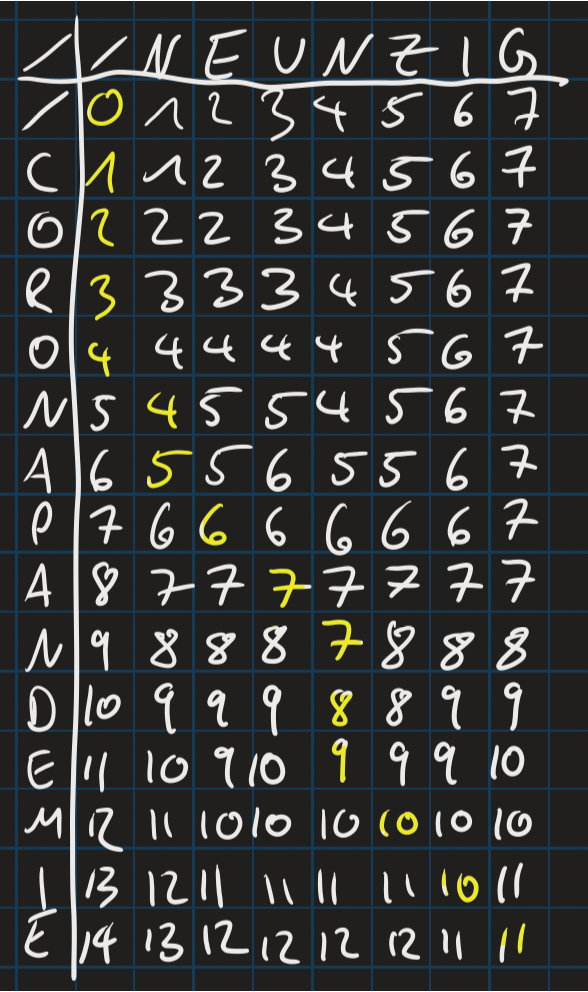
\includegraphics[width=0.4\textwidth]{Bilder/MatrixNormal.png} 
	\caption{Levenshtein-Matrix}
	\label{fig:matrix1}
\end{figure}

\section{Levenshtein Distanz}
\begin{quote}
    Aufbauend auf (a), wie hoch ist die Levenshtein similarity? (siehe Vorlesungsskript)
\end{quote}
Die Levenshtein-Similarity zwischen den Worten ''Coronapandemie'' und ''Neunzig'' liegt zwischen 1 und 0, wobei 1 heißt, dass die beiden Wörter gleich sind. Dadurch lässt sich die Similarity wie folgt berechnen: 
\begin{align*}
    1 - \frac{D}{L}
\end{align*}

$D$: Distanz

$L$: Länge des längsten Wortes

Aus (a) ist die Distanz bekannt. Wird die Distanz sowie die Länge des längsten Wortes (in diesem Fall ''Coronapandemie'') in die Formel eingesetzt, kann die Similarity nun berechnet werden:
\begin{align*}
    1 - \frac{11}{14} = 0,214
\end{align*}

Somit beträgt die Similarity zwischen den beiden Wörtern 0,214 oder 21,4\%

\section{Levenshtein Matrix mit unterschiedlichen Kosten}
\begin{quote}
    In (a) haben wir implizit für das Ersetzen, Hinzufügen und Löschen von Buchstaben Kosten von 1 angenommen. Jetzt ändern wir die Kosten für das Ersetzen eines Buchstabens zu 2. Die Kosten für das Hinzufügen und Löschen bleiben bei 1. Berechne erneut die Levenshtein Distanz des Wortes ''Coronapandemie'' zu deinem Nachnamen mit Hilfe der in der Vorlesung gezeigten Matrix-Methode
\end{quote}
Wenn für das Ersetzen eines Buchstaben Kosten von 2 anfallen, beträgt die Distanz 15. Die Matrix befindet sich in Abbildung \ref{fig:matrix2}.

\clearpage

\begin{figure}[ht]
	\centering
	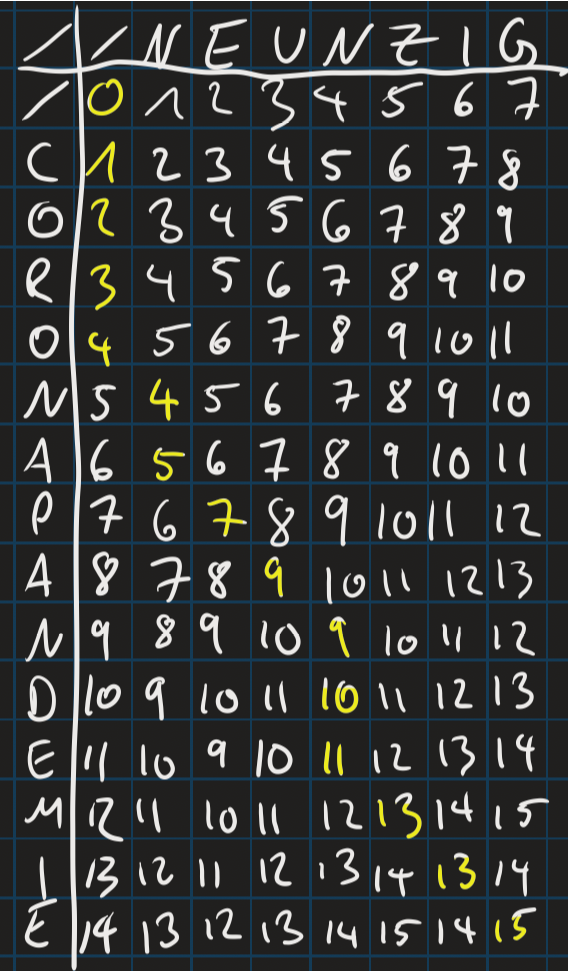
\includegraphics[width=0.4\textwidth]{Bilder/MatrixKosten.png} 
	\caption{Levenshtein-Matrix mit anderen Kosten}
	\label{fig:matrix2}
\end{figure}

\section{Jaccard Distanz}
\begin{quote}
    Berechne die Jaccard similarity des Wortes ''Coronapandemie'' zu deinem Nachnamen auf Basis von 2-grams. Liste dabei auch die jeweiligen 2-grams auf.
\end{quote}
Die Jaccard-Similarity der Wörter beträgt 0. Dies liegt daran, dass es keine übereinstimmenden 2-grams in den jeweiligen Mengen der beiden Wörter gibt: $A \cap B = 0$. Die 2-grams der Wörter ''Neunzig'' und ''Coronapandemie'' lauten wie folgt:

$A = \{NE, EU, UN, NZ, ZI, IG\}$

$B = \{CO, OR, RO, ON, NA, AP, PA, AN, ND, DE, EM, MI, IE\}$



\chapter{HDFS}
\begin{quote}
    Die Sunshine AG ist ein großer Reiseveranstalter und hat im Laufe der Zeit 10 Mio. Bilder von Reisezielen, Hotels, Cafes usw. gesammelt. Im Durchschnitt ist jedes Bild ca. 2 Megabyte groß. Die Bilder werden auf einem einzigen Zentralserver gespeichert. In Zukunft möchte die Sunshine AG auch Bilder und Videos, die sie von ihren Kunden zugesendet bekommt, langfristig abspeichern und erwartet mittelfristig weitere 75 Mio. Dateien á 15 Megabyte.
\end{quote}

\section{Entscheidung für HDFS}
\begin{quote}
    Würde ein HDFS hier Sinn machen? Begründe Deine Antwort mit Deinen eigenen Worten.
\end{quote}
Ein HDFS würde für die Sunshine AG mit derzeitiger technischer Ausrüstung keinen Sinn ergeben. HDFS ist eine einfache und günstige Methode der Datenspeicherung, jedoch nur auf verteilten Systemen, die damit ein hochverfügbares System darstellen können. Durch die momentane technische Ausstattung wäre ein HDFS nicht möglich. 

Wenn die Sunshine AG jedoch neue Hardware kauft und in günstige und mehrere Server investiert, können die vielen Bilder und Dateien dort dann günstig und einfach abgespeichert werden - dann würde sich ein HDFS lohnen. Dort können die Bilder dann in dem HDFS Data Lake gespeichert werden, welches noch aufgesetzt werden müsste. Jedoch sollten die Server bzw. Racks so groß sein, dass dort eine Vielzahl von Dateien drauf abgespeichert werden kann, da die erwarteten Speicherauslastungen sehr groß sind:

    $(10.000.000 * 2 MB = 20.000.000 MB) + (75.000.000 * 15 MB = 1.125.000.000 MB) = 1.145.000.000 MB$
    
Durch die geringen Hardwareanforderungen an HDFS-Server sollte dies jedoch kein Kostenproblem darstellen.

\section{Hochverfügbares HDFS}
\begin{quote}
    Die Sunshine AG entscheidet sich dazu, lediglich die 10 Mio. + 75 Mio. Bilder in einem HDFS zu speichern. Angenommen das HDFS besteht aus 100 Data Nodes, die jeweils eine Ausfallwahrscheinlichkeit von 20 \% besitzen und einem Name Node, der nicht ausfallen kann. Wie oft müssten die Bilder repliziert sein, damit die Sunshine AG eine hochverfügbare Lösung hat? 
\end{quote}
Hochverfügbarkeit bezeichnet in der Literatur eine Eigenschaft von Systemen, die aussagt, dass das System zu 99,9 \% läuft \cite{bundesamt_fur_sicherheit_in_der_informationstechnik_einfuhrung_2013} \cite{portnoy_virtualisierung_2012} \cite{ieee_high_2010}, was auch als Verfügbarkeitsstufe 2 bekannt ist \cite{frey_hochverfugbarkeit_2010}. Das bedeutet, dass das System für 8:45:58 Stunden pro Jahr ausfallen darf. Je nach Literatur oder Hersteller von Produkten kann Hochverfügbarkeit auch erst ab 99,99 \% gegeben sein \cite{frey_hochverfugbarkeit_2010}. Das würde einer Downtime von 52:36 Minuten pro Jahr entsprechen. Da es sich in der Aufgabe um Bilder bei einem Reiseveranstalter handelt, kann 99,9 \% Uptime als hochverfügbar genommen werden. 

Um eine Verfügbarkeit von 99,9 \% zu gewährleisten, müssen die Bilder auf verschiedenen Servern repliziert werden, damit immer auf einen Server zugegriffen werden kann, der nicht ausfällt. 
\begin{align*}
    0,2^x <= 0,001
\end{align*}
\begin{align*}
    x \cdot log(0,2) >= log(0,001)
\end{align*}
\begin{align*}
    x >= \frac{log(0,001)}{log(0,2)}
\end{align*}
\begin{align*}
    x >= 4,292
\end{align*}

$x$: Anzahl an Name Nodes, auf denen ein Bild repliziert werden muss

$0,2$: Ausfallwahrscheinlichkeit einer Name Node $1 - 0,8$

$0,001$: Erlaubte Ausfallwahrscheinlichkeit bei Hochverfügbarkeit $1 - 0,999$

Nach der Berechnung müssen die Bilder demnach auf mehr als 4,292 Name Nodes repliziert werden, was aufgerundet mindestens 5 Name Nodes entspricht, damit Hochverfügbarkeit der Bilder im System gegeben wird. Würde als Hochverfügbarkeitsdefinition 99,99 \% in Betracht gezogen werden, würde sich in den Rechnungen die Ausfallwahrscheinlichkeit von 0,001 auf 0,0001 verringern. Dann beträge x = 5,723 und man bräuchte eine 6-fache Replikation der Bilder auf den Name Nodes.

\chapter{Processing Frameworks}

\section{MapReduce}
\begin{quote}
    MapReduce wird heute nur noch selten für die Verarbeitung von sehr großen Datensätzen genutzt. Warum? Begründe mit Deinen eigenen Worten.
\end{quote}

MapReduce hat viele Vorteile, wenn es um die Verarbeitung von Datensätzen geht. Jedoch gibt es einige Nachteile, die heutzutage einfach durch andere Programme ausgeglichen werden können. Zum einen folgt MapReduce immer dem selben Ablauf Map, Shuffle und Reduce. Für Anforderungen, wo weitere Operationen und Transformationen nötig sind, ist dies nicht sinnvoll. Außerdem ist MapReduce recht langsam. MapReduce nutzt nämlich die Festplatte und keinen Cache, weshalb dauerhaft Disk-Operationen genutzt werden. Andere Programme, die mit Cache oder RAM arbeiten, sollten dort eher eingesetzt werden. 

\section{MapReduce in Java}
\begin{quote}
    Gegeben ist folgendes MapReduce Programm, geschrieben in Java:
\end{quote} 
\lstinputlisting[
    language=Java,
	caption=Vorgegebener Code für Aufgabe 3b,
	captionpos=t,               % Position, an der die Caption angezeigt wird t(op) oder b(ottom)
	firstline=1,                % Zeilennummer im Dokument welche als erste angezeigt wird
	lastline=24              % Letzte Zeile welche ins LaTeX Dokument übernommen wird
]{Quellcode/3b.java}
\begin{quote}
    Erstelle nun zwei Texte. Der erste Text besteht aus deinem Vor- und Nachnamen. Der zweite Text besteht aus Deinem Wohnort und Arbeitgeber, z.B.: Text1: Alexander Lütke; Text2: Düsseldorf IBM Deutschland GmbH. Nutze diesen Text als Input für das oben gegebene MapReduce-Programm. Schreibe auf, welchen Output das Programm nach der Map-, nach der Shuffle- und nach der Reduce-Phase jeweils erzeugt. Übernimm‘ dabei das Format aus der Vorlesung.
\end{quote}
Die beiden Texte für die Aufgabe lauten ''Mathis Neunzig'' und ''Mannheim SAP SE''. Wenn diese Texte durch die Map-, Shuffle- und Reduce-Phase des gegebenen Programms laufen, ergeben sich folgende Ergebnisse:

\subsubsection{Input}
\lstinputlisting[
    language=Java,
	caption=Input für Aufgabe 3b und 3c,
	captionpos=t,               % Position, an der die Caption angezeigt wird t(op) oder b(ottom)
	firstline=1,                % Zeilennummer im Dokument welche als erste angezeigt wird
	lastline=2             % Letzte Zeile welche ins LaTeX Dokument übernommen wird
]{Quellcode/Input.java}

\subsubsection{Map}
\lstinputlisting[
    language=Java,
	caption=Ausgabe Map-Phase,
	captionpos=t,               % Position, an der die Caption angezeigt wird t(op) oder b(ottom)
	firstline=1,                % Zeilennummer im Dokument welche als erste angezeigt wird
	lastline=29              % Letzte Zeile welche ins LaTeX Dokument übernommen wird
]{Quellcode/Map.java}

\subsubsection{Shuffle}
\lstinputlisting[
    language=Java,
	caption=Ausgabe Shuffle-Phase,
	captionpos=t,               % Position, an der die Caption angezeigt wird t(op) oder b(ottom)
	firstline=1,                % Zeilennummer im Dokument welche als erste angezeigt wird
	lastline=4             % Letzte Zeile welche ins LaTeX Dokument übernommen wird
]{Quellcode/Shuffle.java}

\subsubsection{Reduce}
\lstinputlisting[
    language=Java,
	caption=Ausgabe Reduce-Phase,
	captionpos=t,               % Position, an der die Caption angezeigt wird t(op) oder b(ottom)
	firstline=1,                % Zeilennummer im Dokument welche als erste angezeigt wird
	lastline=4             % Letzte Zeile welche ins LaTeX Dokument übernommen wird
]{Quellcode/Reduce.java}

\section{MapReduce mit Spark}
\begin{quote}
    Transformiere das oben gegebene MapReduce Programm in ein Spark Programm.
\end{quote}
Die nachfolgende Java-Datei befindet sich zusätzlich in der Abgabe auf Moodle.
\lstinputlisting[
    language=Java,
	caption=Ergebnis Aufgabe 3c,
	captionpos=t,               % Position, an der die Caption angezeigt wird t(op) oder b(ottom)
	firstline=1,                % Zeilennummer im Dokument welche als erste angezeigt wird
	lastline=76             % Letzte Zeile welche ins LaTeX Dokument übernommen wird
]{Quellcode/3c.java}

\chapter{Cloud}

\section{Nutzung von Cloud-Systemen}
\begin{quote}
    Welche Gründe sprechen für die Nutzung von Cloud-Systemen?
\end{quote}
Für eine Nutzung von Cloud-Systemen sprechen mehrere Gründe. Zum einen geben Cloud-Systeme die Möglichkeit, dass Software, Infrastrukturen und Plattformen als Service angeboten werden, welche der Anwender abonnieren kann. Dadurch entfallen Kosten für Wartung und Hardware, es fallen lediglich Kosten für das Abonnement an. Cloud-Systeme sind auch von überall ansprechbar. Das bedeutet, dass man zum Arbeiten mit diesen Systemen von überall auf dieses zugreifen kann. Die Daten in Cloud Systemen sind oft, jedoch nicht immer, geographisch verteilt. Damit liegen die Daten auf verschiedenen Servern, die zusammen eine geringere Ausfallquote haben, als ein einzelnes on-Premise-System.

\section{On-Premise vs. Cloud}
\begin{quote}
    In welchem Fall würdest Du ein Hadoop-System on-Premise aufsetzen, wann hingegen in der Cloud?
\end{quote}
Ein Hadoop-System in der Cloud lohnt sich vor allem, wenn ein System mit einer hohen Flexibilität und Skalierbarkeit gewünscht ist. Durch die Vorteile von Cloud-Systemen, wo man die Ressourcen zahlt und bekommt, die man auch nutzt, können Schwankungen in der Nutzung abgefangen werden. Zusätzlich ist das Cloud-System, wie in Aufgabe 4a) beschrieben, günstiger, da keine eigenen Hardware- und Wartungskosten anfallen. Zusätzlich sind die Daten in der Cloud möglicherweise auf verschiedenen Systemen gespeichert, die ausfalltechnisch und lokationstechnisch unabhängig voneinander sind, was dem System eine höhere Ausfalltolleranz gibt. 

Ein On-Premise-Hadoop-System lohnt sich vor allem, wenn es einen konstanten hohen Speicherbedarf gibt, da somit die Daten direkt zur Hand sind, wenn diese gebraucht werden. Wenn es hohe Sicherheitsanforderungen gibt, macht es auch Sinn, ein on-Premise-System anzuschaffen. Dieses ist sicherheitstechnisch komplett konfigurierbar und kann an alle Sicherheitsanforderungen angepasst werden.

\section{AWS Glue}
\begin{quote}
    Welche Verantwortung für die Sicherheit einer ''AWS Glue''-Anwendung übernimmt ein Cloud-Provider laut des ''Shared Responsibility Model''? Welche Verantwortung übernimmt demnach der Cloud-Kunde?
\end{quote}
Bei AWS Glue übernimmt AWS als Teil des ''Shared Responsibility Models'' selber einen Teil der Verantwortung der Sicherheit. Darunter zählt die Sicherheit der Infrastruktur selber, die AWS bereitstellt. Dazu gehören zum Beispiel auch die Rechenzentren von AWS, die als AWS Glue abonniert werden sowie die Authentifizierung des Anwenders bei AWS. Des Weiteren ist es die Pflicht von AWS, sich um die Sicherheit des AWS Glue Dienstes zu kümmern, wozu die Authentifizierung am Dienst sowie die Datenverschlüsselung gehören. 

Der Anwender selber hat dazu andere Verpflichtungen, wie zum Beispiel das Managen von Upgrades und Patches, die Sicherheitsüberwachung und Konfiguration des Services. Zusätzlich muss sich der Anwender um die Datenverwaltung und den Datenschutz der eigenen Daten kümmern, wozu auch die Zugriffssteuerung von Daten gehört. 

\section{AWS Glue ETL}
\begin{quote}
    Würdest du ''AWS Glue ETL'' als eine Software-as-a-Service, Platform-as-a-Service, oder Infrastructure-as-a-Service bezeichnen? Begründe deine Antwort mit deinen eigenen Worten.
\end{quote}
AWS Glue ETL ist ein Platform-as-a-Service, da der Anwender bei der Nutzung des ETL-Dienstes keinen direkten Zugriff auf die Infrastruktur hat, sondern die von AWS bereitgestellte Plattform nutzt. Auf dieser Plattform können dann die ETL-Jobs ausgeführt werden. Die Infrastruktur, auf der AWS Glue läuft, ist von AWS bereitgestellt und gehört auch nicht per se zum Abonnement, jedoch die daraufliegende Plattform. Bei AWS Glue ETL handelt es sich auch nicht um Software-as-a-Service, da keine Standardsoftware für die breite Masse angeboten wird. 

% ---- Literaturverzeichnis
\cleardoublepage
\renewcommand*{\chapterpagestyle}{plain}
\pagestyle{plain}
\pagenumbering{Roman}                   % Römische Seitenzahlen
\setcounter{page}{\numexpr\value{savepage}+1}
\printbibliography[title=Literaturverzeichnis]

% ---- Anhang
%\clearpage
%\pagenumbering{Roman}  % römische Seitenzahlen für Anhang

\newpage
\end{document}
